\documentclass{standalone}
\usepackage{tikz}
\usetikzlibrary{positioning, shapes, arrows, shadows}

\begin{document}
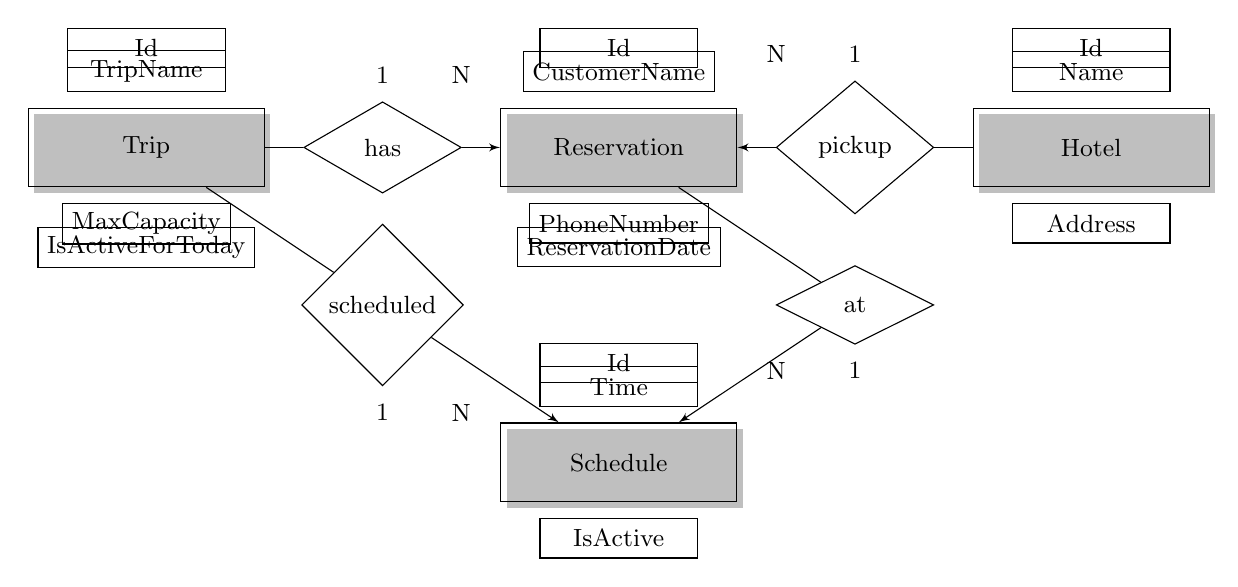
\begin{tikzpicture}[
    entity/.style={rectangle, draw, minimum width=3cm, minimum height=1cm, drop shadow},
    attribute/.style={rectangle, draw, minimum width=2cm, minimum height=0.5cm},
    relationship/.style={diamond, draw, minimum width=2cm, minimum height=1cm},
    line/.style={draw, -latex'},
    every node/.style={font=\small}
]

% Entities
\node[entity] (trip) at (0,0) {Trip};
\node[entity] (reservation) at (6,0) {Reservation};
\node[entity] (hotel) at (12,0) {Hotel};
\node[entity] (schedule) at (6,-4) {Schedule};

% Trip attributes
\node[attribute] (trip_id) [above=0.5cm of trip] {Id};
\node[attribute] (trip_name) [above=0.2cm of trip] {TripName};
\node[attribute] (trip_capacity) [below=0.2cm of trip] {MaxCapacity};
\node[attribute] (trip_active) [below=0.5cm of trip] {IsActiveForToday};

% Reservation attributes
\node[attribute] (res_id) [above=0.5cm of reservation] {Id};
\node[attribute] (res_customer) [above=0.2cm of reservation] {CustomerName};
\node[attribute] (res_phone) [below=0.2cm of reservation] {PhoneNumber};
\node[attribute] (res_date) [below=0.5cm of reservation] {ReservationDate};

% Hotel attributes
\node[attribute] (hotel_id) [above=0.5cm of hotel] {Id};
\node[attribute] (hotel_name) [above=0.2cm of hotel] {Name};
\node[attribute] (hotel_address) [below=0.2cm of hotel] {Address};

% Schedule attributes
\node[attribute] (sch_id) [above=0.5cm of schedule] {Id};
\node[attribute] (sch_time) [above=0.2cm of schedule] {Time};
\node[attribute] (sch_active) [below=0.2cm of schedule] {IsActive};

% Relationships
\node[relationship] (trip_res) at (3,0) {has};
\node[relationship] (hotel_res) at (9,0) {pickup};
\node[relationship] (trip_sch) at (3,-2) {scheduled};
\node[relationship] (res_sch) at (9,-2) {at};

% Lines
\draw[line] (trip) -- (trip_res) -- (reservation);
\draw[line] (hotel) -- (hotel_res) -- (reservation);
\draw[line] (trip) -- (trip_sch) -- (schedule);
\draw[line] (reservation) -- (res_sch) -- (schedule);

% Cardinality
\node[above=0.1cm of trip_res] {1};
\node[above=0.1cm of hotel_res] {1};
\node[below=0.1cm of trip_sch] {1};
\node[below=0.1cm of res_sch] {1};

\node[above=0.1cm of trip_res, xshift=1cm] {N};
\node[above=0.1cm of hotel_res, xshift=-1cm] {N};
\node[below=0.1cm of trip_sch, xshift=1cm] {N};
\node[below=0.1cm of res_sch, xshift=-1cm] {N};

\end{tikzpicture}
\end{document} 